%!TEX root = ../main.tex
\chapter{Le projet et son impact sur les équipes}
Comme pour tout projet lié à des éléments de l'architecture informatique d'une entreprise, la sécurisation de la chaîne
de production d'applications conteneurisées à un impact sur différentes équipes de l'entreprise. Cet impact est présent
tant lors de la mise en place du projet dès la phase opérationnelle faisant suite à la livraison du projet.

Nous chercherons donc dans ce chapitre à évaluer cet impact sur les équipes du Groupe ainsi que les éventuelles 
difficultés rencontrées durant la réalisation de ce projet.

\section{Rappel de contexte}
Comme évoqué dans les précédemment chapitres, cette mission de fin d'étude et le projet associé s'est déroulé
durant la crise de la COVID-19, plus particulièrement de la \textit{3ᵉ vague épidémiologique}. Cette crise ayant un 
impact mondial, les activités du Groupe JCDecaux ont significativement baissées. Une majorité des unités organisationnelles
ont donc vue leur activité réduite à divers pourcentages.

Cette réduction d'activité, à hauteur de 30\% pour la \ac{DSI} Groupe et les départs liés aux deux plans de conservation
de l'emploi ont eu pour effet de mettre en tension les équipes de la \ac{DSI}. Ainsi, si en théorie cette mission est
censé représenter six mois de travail, dans les faits elle représente un peu plus de trois mois effectifs.
\newline De plus, l'activité de l'équipe sécurité ainsi que celle des autres équipes impactées par ce projet n'étant pas 
pas arrêter, mais modérément diminué. Ce projet ne pouvait donc occuper 100\% du temps de travail.

Ces éléments expliquent donc la durée de réalisation de cette mission qui, à mon sens, aurait pu être réalisé en 
quatre mois dans des conditions plus favorables.

\section{Évaluation des charges et rétroplanning}
Ce projet a été réalisé en deux phases successives : une première phase visant à entériner la procédure de qualification 
sécurité des applications puis une deuxième visant à sécuriser les conteneurs et leur déploiement sur \ac{K8S}.
\newline Plusieurs équipes de la \ac{DSI} ont participé à la réalisation de ce projet conjointement avec l'équipe de 
\ac{SSI}.

\newpage

La charge pour ces équipes pour chaque grandes étapes du projet est estimée comme suivant :
\begin{enumerate}
    \item Processus d'audit :
    \begin{itemize}
        \renewcommand{\labelitemi}{•}
        \item Équipes de développement France : 13 équ. Heure/Homme
    \end{itemize}
    \item Sécurisation des clusters \ac{K8S} :
    \begin{itemize}
        \renewcommand{\labelitemi}{•}
        \item Équipe d'architecture : 27 équ. Heure/Homme
        \item Équipe d'infrastructure : 5 équ. Heure/Homme
    \end{itemize}
    \item Politique de sécurité \ac{K8S} :
    \begin{itemize}
        \renewcommand{\labelitemi}{•}
        \item Équipe d'architecture : 3 équ. Heure/Homme
        \item Équipes d'infrastructure : 6 équ. Heure/Homme
    \end{itemize}
    \item Revue des vulérabilités des conteneurs :
    \begin{itemize}
        \renewcommand{\labelitemi}{•}
        \item Équipes d'architecture : 1 équ. Heure/Homme
        \item Équipes d'infrastructure : 5+ équ. Heure/Homme
    \end{itemize}
\end{enumerate}

Cette mission de fin d'étude ne disposant pas de réelles contraintes temporelles, seuls quelques jalons ont été proposés.
C'est pourquoi j'ai réalisé un rétroplanning afin de vous présenter la chronologie du projet.

\begin{figure}[h]
    \centering
    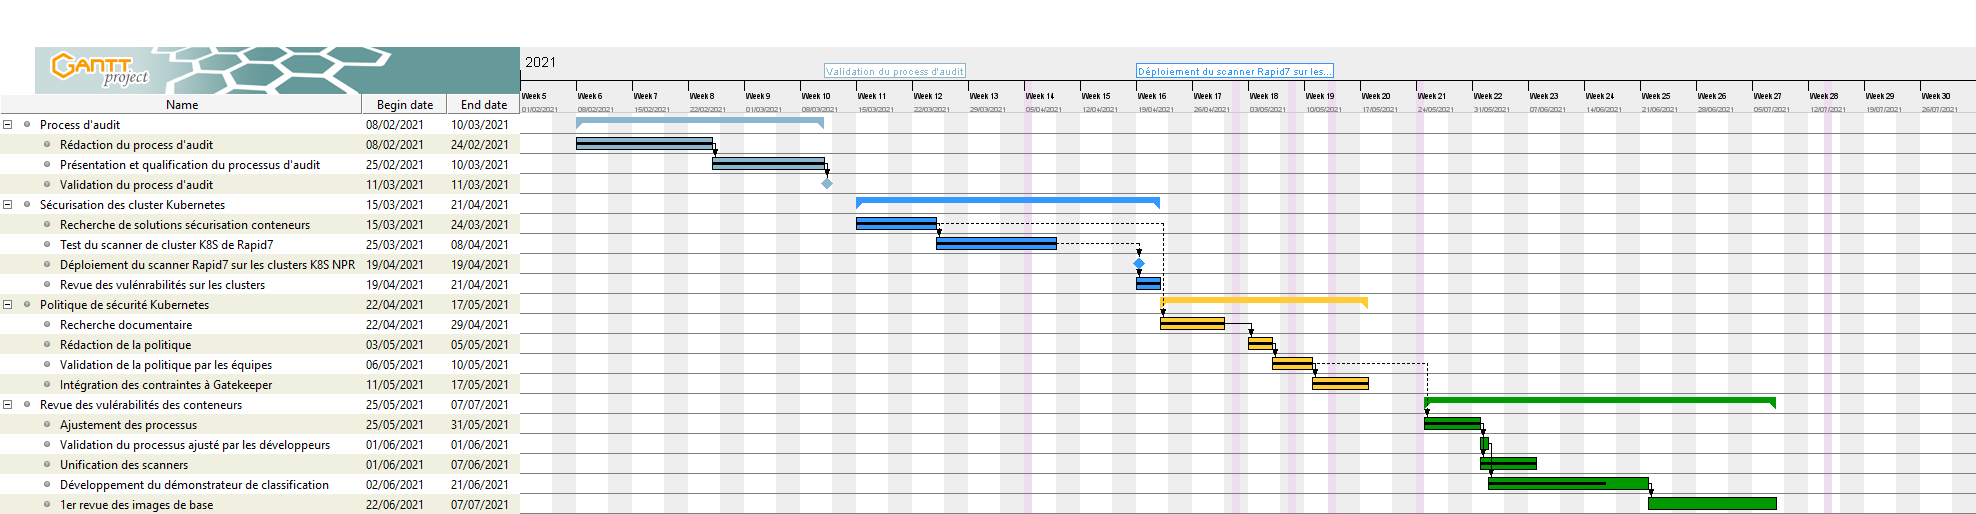
\includegraphics[width=\linewidth]{resources/img/retroplanning.png}
    \caption{Rétroplanning de la mission de fin d'étude}
\end{figure}

\begin{center}
    \colorbox{gray!15}{Une version plus lisible est disponible dans les annexes}
\end{center}

\newpage

\section{Estimation de l'impact du projet}
Compte tenu des modifications que nous avons apportées à l'infrastructure \ac{K8S} et aux processus de développement,
on peut sans difficultés imaginer que ce projet aura un impact notable sur le fonctionnement des équipes du Groupe 
JCDecaux et leur façon d'interagir entre elles.
\newline Nous allons donc tenter d'estimer cet impact pour chacune des équipes embarquées dans ce projet.

\subsection{Pour les équipes de développement}
Les équipes de développement vont faire partie des équipes les plus impactées par ce \linebreak projet.
Si elles n'étaient que peu associées à la gestion de la sécurité des développements (rappel: elles n'étaient sollicitées que
lors d'audit applicatif), l'intégration de la sécurisation des conteneurs dans leur processus va avoir un impact 
significatif.
\newline On peut en effet estimer que ces nouvelles actions vont représenter à minima 4 équ. Heures/Homme par sprint.

Cependant, cette estimation ne sera valable qu'après une première phase de rodage et de réduction du bruit des outils
grâce à la mise en place des AllowList de vulnérabilités.
\newline L'équipe chargée du maintien et du développement des images \emph{de base} se verra pendant cette première phase 
largement impactée (3 à 4 équ. Jours/Homme) du fait qu'elle devra mettre à jour et corriger toutes les images 
\emph{de base}. 

\subsection{Pour les équipes opérationnelles}
Nous n'avons pas beaucoup parlé de ces équipes dans ce mémoire, et pour cause; elles ne devraient être que marginalement 
impactées par les modifications apportées par ce projet.

En effet, si le travail réalisé par ces équipes est primordiale au bon fonctionnement des clusters \ac{K8S}, ces dernières
ne verront pas de changement significatif dans leurs processus opérationnels ni dans leurs outils.
\newline On peut donc estimer que l'impact du projet pour ces équipes est non significatif et donc nulle.

\subsection{Pour l'équipe d'architecture}
Le travail de l'équipe d'architecture a été d'une grande importance durant ce projet et cela se reflète sur le temps 
qu'elle nous a allouée. Cependant, une fois les processus en place et les outils opérationnels et configurés, elle ne 
devrait plus être impactée par les solutions mises en œuvre dans ce mémoire. Du moins, tel en est l'objectif.

Nous pouvons donc aisément estimer qu'elle devrait passer que 2 à 3 équ. Heure/Homme par trimestre, pour implémenter
de nouvelles règles sur l'\emph{OPA Gatekeeper} ou extraire quelques informations au profit de l'équipe de \ac{SSI}.

\subsection{Pour l'équipe de sécurité informatique}
Si l'on devait désigner un perdant au jeu des impacts, l'équipe de \ac{SSI} serait sans aucun doute désignée perdante.
\newline En effet les modifications apportées aux processus de gestion de la sécurité lui ont rajouté certaines prérogatives
et un nombre certain de nouvelles tâches.

Ainsi, avec l'intégration de \ac{K8S} aux actions de gestions opérationnelle de la sécurité des infrastructures, 
la modification du processus d'audit et surtout la mise en place de revue de vulnérabilité pour les conteneurs,
l'équipe de \ac{SSI} se vera fortement impactée par ce projet.
\newline On peut sans trop de réserve estimer que ces nouvelles charges représenteront 7 à 10 équ. Jour/Homme.